\documentclass[aspectratio=169]{beamer}

% ── Theme ────────────────────────────────────────────────────────────────────
\usetheme{CambridgeUS}
\usecolortheme{beaver}
\setbeamertemplate{navigation symbols}{}
\setbeamertemplate{footline}[frame number]
\setbeamerfont{title}{size=\large}
\setbeamerfont{frametitle}{size=\normalsize}

% ── Packages ─────────────────────────────────────────────────────────────────
\usepackage{graphicx}
\usepackage{booktabs}
\usepackage{array}
\usepackage{xcolor}
\usepackage{tikz}
\usepackage{hyperref}

% ── Colours ──────────────────────────────────────────────────────────────────
\definecolor{myblue}{HTML}{2166AC}
\definecolor{myred}{HTML}{D6604D}
\definecolor{mygreen}{HTML}{4DAC26}
\definecolor{mygray}{HTML}{888888}

% ── Figure path ──────────────────────────────────────────────────────────────
\graphicspath{{../output/figures/}}

% ── Title info ───────────────────────────────────────────────────────────────
\title{Federal Economist Compensation \& PhD Placement:\\
       Evidence by Gender}
\subtitle{Updated Data and New Sources}
\author{Danielle H.\ Sandler}
\institute{U.S.\ Census Bureau}
\date{\today}

% ─────────────────────────────────────────────────────────────────────────────
\begin{document}

\begin{frame}
  \titlepage
\end{frame}

% ── Outline ──────────────────────────────────────────────────────────────────
\begin{frame}{Outline}
  \tableofcontents
\end{frame}

% =============================================================================
\section{Overview and Data}
% =============================================================================

\begin{frame}{Overview}
  \textbf{This project extends prior work on gender equity among economists in two ways:}
  \begin{enumerate}
    \item Updates the federal salary analysis through FY2024 using FedsDataCenter
          (previously through FY2015 in Foster, Manzella, McEntarfer \& Sandler 2020)
    \item Introduces a new data source on PhD economist initial placements
          (44 programs, 1991--2025) to complement the LEHD-based analysis
          in Foster, McEntarfer \& Sandler (2023)
  \end{enumerate}
  \vspace{0.5em}
  \textbf{Key questions:}
  \begin{itemize}
    \item How has the federal economist gender pay gap evolved since 2015?
    \item How do initial placement shares compare across sectors and over time?
    \item How does the gender composition of placements compare to the full SED/LEHD sample?
  \end{itemize}
\end{frame}

\begin{frame}{Data Sources}
  \begin{columns}
    \begin{column}{0.5\textwidth}
      \textbf{Federal salary data}\\[0.4em]
      \begin{itemize}
        \item Source: FedsDataCenter.com (OPM data via FOIA)
        \item Years: FY2015--FY2024
        \item $\approx$4,300--4,700 economists per year
        \item Occupation code: ``Economist''
        \item Fields: name, agency, grade, pay plan, salary, bonus
        \item Gender assigned via \texttt{gender\_guesser}
              (offline, $\approx$84\% coverage)
      \end{itemize}
    \end{column}
    \begin{column}{0.5\textwidth}
      \textbf{PhD placement data}\\[0.4em]
      \begin{itemize}
        \item Source: econphdplacements.com
        \item 8,824 placements from 44 programs
        \item Includes US and international programs\\
              (e.g., Stockholm, UBC, LSE)
        \item Years: 1991--2025
        \item Fields: name, year, program, field, placement, category
        \item Gender assigned via \texttt{gender\_guesser}
              ($\approx$51\% coverage)
      \end{itemize}
    \end{column}
  \end{columns}
\end{frame}

\begin{frame}{A Note on Gender Assignment}
  Both datasets use \textbf{name-based gender assignment} via \texttt{gender\_guesser}
  (an offline library covering $\approx$40,000 names):
  \vspace{0.5em}
  \begin{itemize}
    \item Returns: \textit{male}, \textit{mostly\_male}, \textit{female}, \textit{mostly\_female},
          \textit{androgynous}, \textit{unknown}
    \item We assign male/female from the first two; leave the rest unassigned
    \item Salary data: \textbf{84\%} coverage (OPM names are mostly Anglo-American)
    \item Placement data: \textbf{51\%} coverage (many international names not in library)
    \item Unassigned names skew international and likely male-heavy
          $\Rightarrow$ female shares in placement data are \textit{understated}
    \item Prior papers (Foster et al.\ 2020, 2023) use \textbf{self-reported} SED gender
          (100\% coverage, no bias)
  \end{itemize}
\end{frame}

% =============================================================================
\section{Federal Salary Analysis}
% =============================================================================

\begin{frame}{Median Salary by Gender, FY2015--2024}
  \begin{center}
    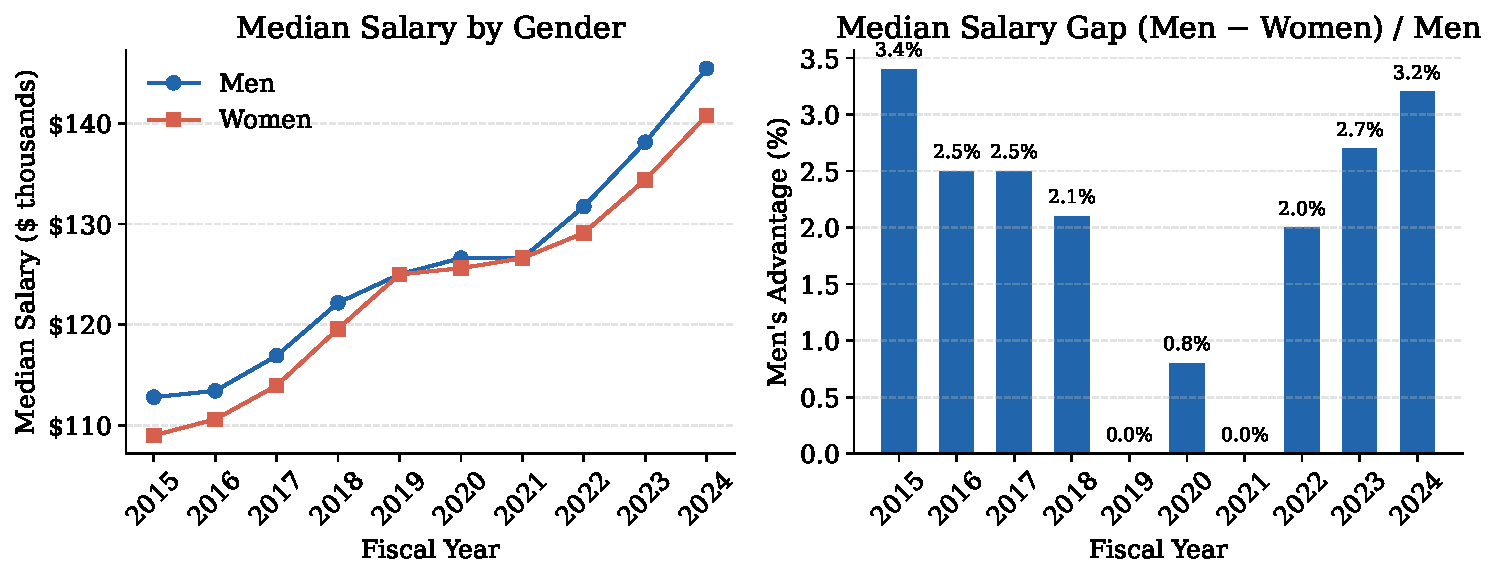
\includegraphics[width=0.92\textwidth]{salary_trends}
  \end{center}
  \begin{itemize}
    \item Gap peaked at 3.4\% in 2015, nearly closed in 2019--2021,
          then \textbf{re-widened to 3.2\%} by 2024
    \item 2024 medians: men \$145,489 \quad women \$140,807
  \end{itemize}
\end{frame}

\begin{frame}{Female Share of Federal Economists by Agency}
  \begin{center}
    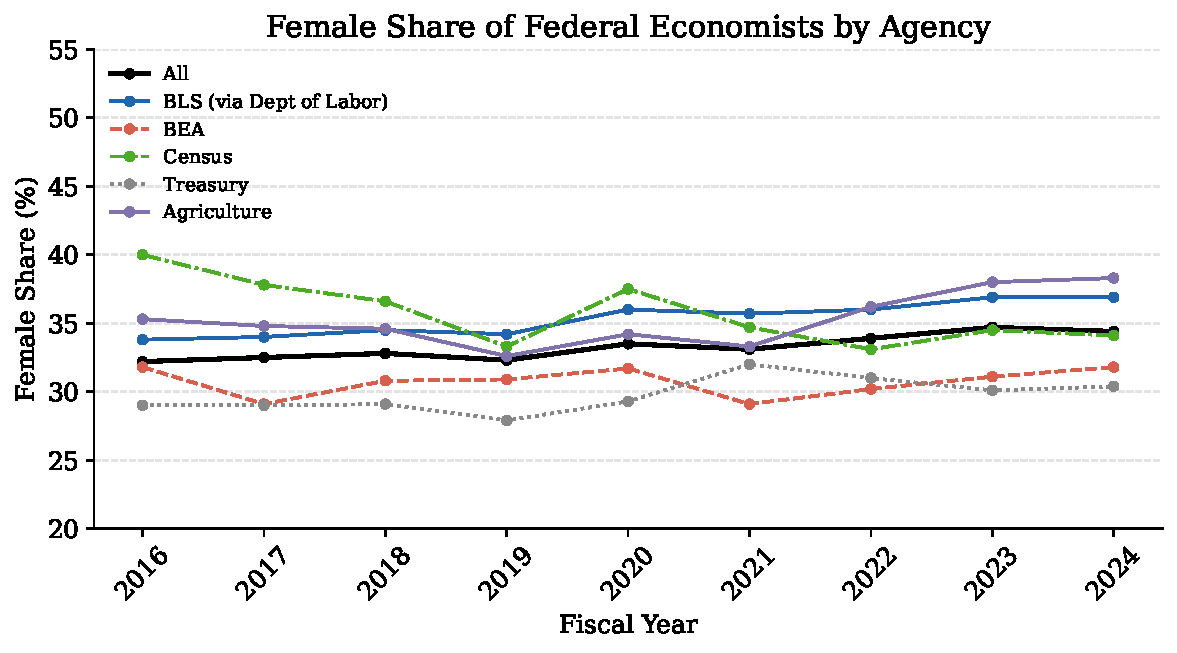
\includegraphics[width=0.90\textwidth]{female_share_agency}
  \end{center}
  \begin{itemize}
    \item Overall share rising: 32\% (2016) $\to$ 34\% (2024)
    \item HHS consistently highest ($\approx$40--45\%); Treasury lowest ($\approx$29--32\%)
  \end{itemize}
\end{frame}

\begin{frame}{Is the Gap Within or Between Grade?}
  \begin{center}
    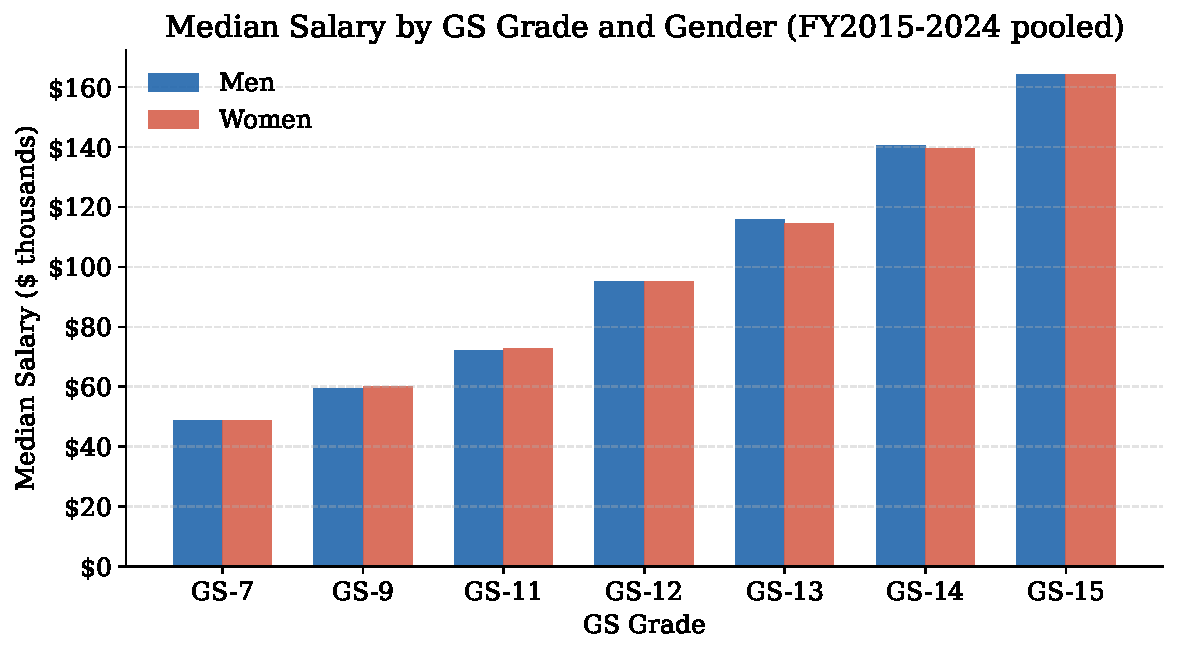
\includegraphics[width=0.88\textwidth]{grade_salary}
  \end{center}
  \begin{itemize}
    \item Within-grade gaps are \textbf{near zero or reversed} across all GS levels
    \item The overall salary gap is driven by \textbf{grade distribution}:
          women are concentrated at lower GS grades
  \end{itemize}
\end{frame}

\begin{frame}{Salary Gap by Agency}
  \begin{center}
    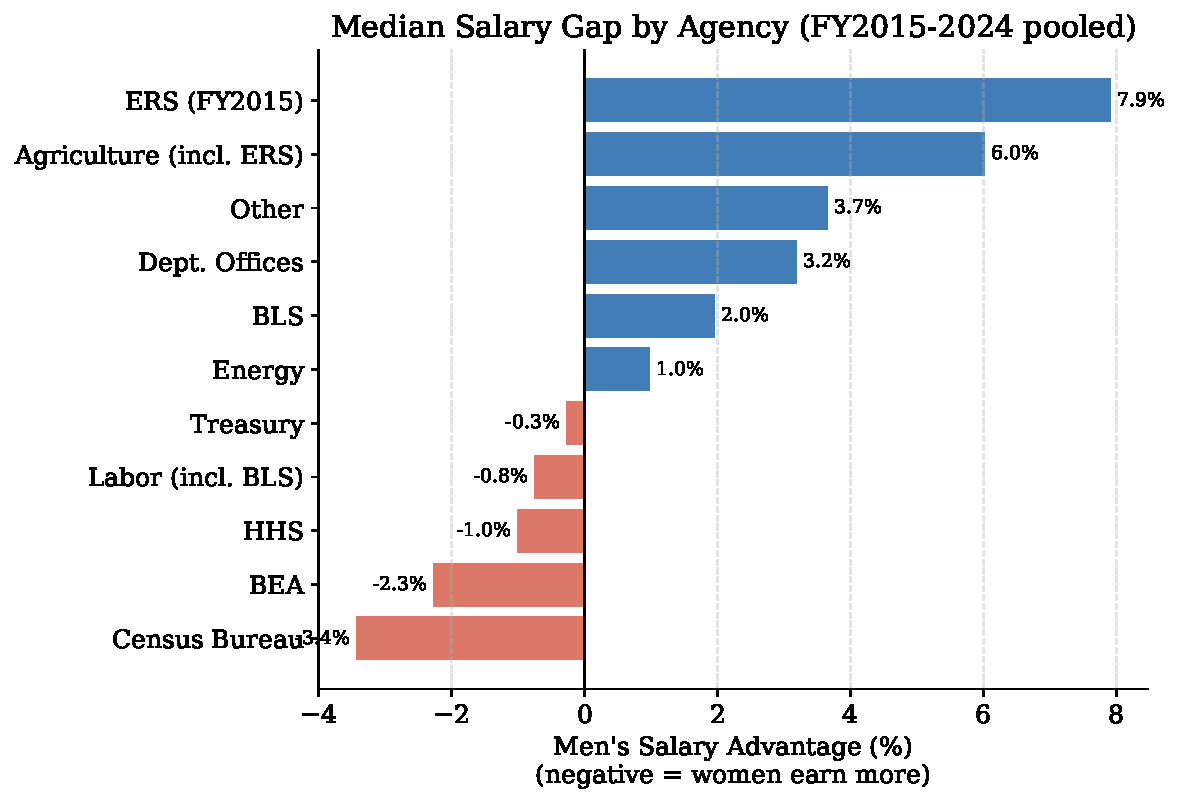
\includegraphics[width=0.88\textwidth]{agency_gap}
  \end{center}
  \begin{itemize}
    \item \textcolor{myred}{BEA, Census Bureau, and BLS show female salary advantage}
          (women earn more at median)
    \item Largest male advantage: Agriculture/ERS and ``Other'' agencies
    \item Pattern consistent with within-grade gaps being near zero:
          agency differences reflect grade composition
  \end{itemize}
\end{frame}

% =============================================================================
\section{Comparison to Prior Work}
% =============================================================================

\begin{frame}{Federal Salary Gap: FedsDataCenter vs.\ Foster et al.\ (2020)}
  \begin{center}
    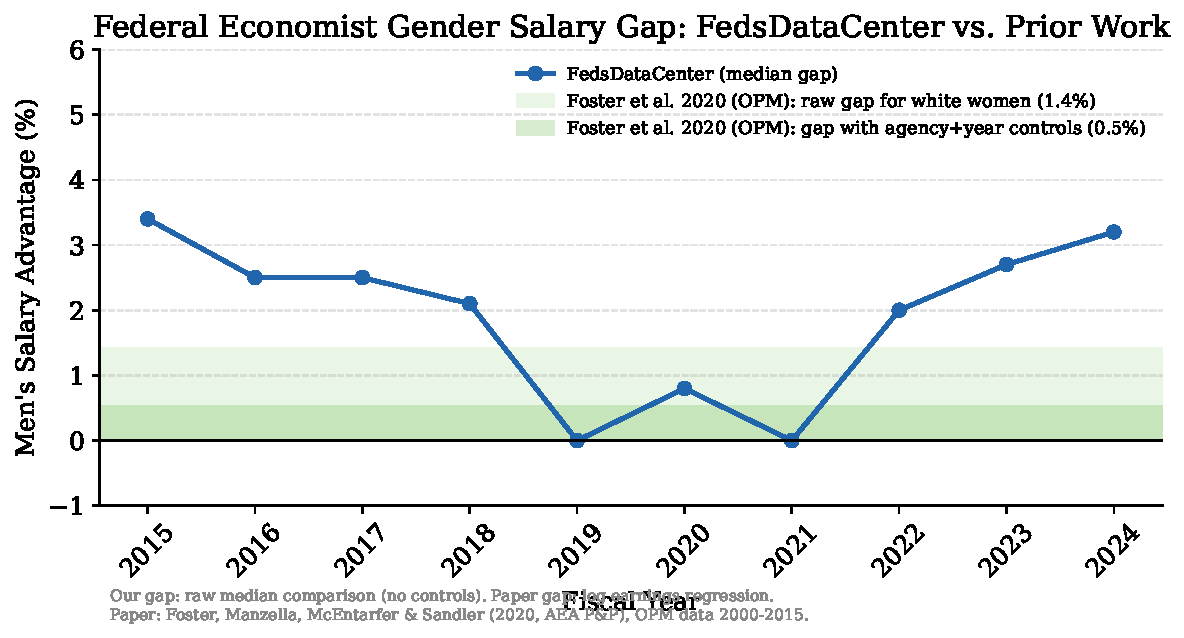
\includegraphics[width=0.88\textwidth]{salary_comparison_paper}
  \end{center}
\end{frame}

\begin{frame}{Federal Salary Gap: Comparison Summary}
  \begin{center}
    \small
    \begin{tabular}{llll}
      \toprule
      Source & Sample & Specification & Gap \\
      \midrule
      FedsDataCenter (FY2015)  & All GS economists & Raw median & 3.4\% \\
      FedsDataCenter (FY2024)  & All GS economists & Raw median & 3.2\% \\
      FedsDataCenter (FY2019--21) & All GS economists & Raw median & $\approx$0\% \\
      \midrule
      Foster et al.\ (2020) & PhD economists, OPM & Raw log gap (white women) & 1.4\% \\
      Foster et al.\ (2020) & PhD economists, OPM & Agency + year FE & 0.5\% \\
      \midrule
      Foster et al.\ (2023) & PhD economists, LEHD & Raw log gap, government & 8.6\% \\
      Foster et al.\ (2023) & PhD economists, LEHD & Full controls, government & 3.8\% \\
      \bottomrule
    \end{tabular}
  \end{center}
  \vspace{0.3em}
  \small
  \begin{itemize}
    \item Our raw 3\% median gap vs.\ OPM-based 1.4\% raw log gap: broadly consistent
    \item LEHD-based 8.6\% is larger because it is \textbf{PhD-only} and captures broader
          compensation (not just base salary)
  \end{itemize}
\end{frame}

% =============================================================================
\section{PhD Placement Analysis}
% =============================================================================

\begin{frame}{PhD Economist Placement Data: Overview}
  \begin{columns}
    \begin{column}{0.48\textwidth}
      \textbf{Sample characteristics}\\[0.4em]
      \begin{itemize}
        \item 8,824 placements, 44 programs
        \item Placement years: 1991--2025
        \item Includes international programs:\\
              Stockholm, UBC, LSE, Sciences Po,\\
              Mannheim, EUI, CEMFI, \ldots
        \item 7 placement categories:\\
              tenure-track, other academic,\\
              private sector, central banks,\\
              government, think tanks,\\
              international orgs
      \end{itemize}
    \end{column}
    \begin{column}{0.48\textwidth}
      \textbf{Overall placement distribution}\\[0.3em]
      \small
      \begin{tabular}{lr}
        \toprule
        Category & Share \\
        \midrule
        Tenure-track & 49.4\% \\
        Private sector & 18.8\% \\
        Other academic & 12.2\% \\
        Central banks & 7.2\% \\
        International orgs & 4.6\% \\
        Think tanks & 3.8\% \\
        Government & 4.1\% \\
        \bottomrule
      \end{tabular}\\[0.4em]
      \textit{Academia total: 61.6\%}
    \end{column}
  \end{columns}
\end{frame}

\begin{frame}{Placement Trends Over Time}
  \begin{center}
    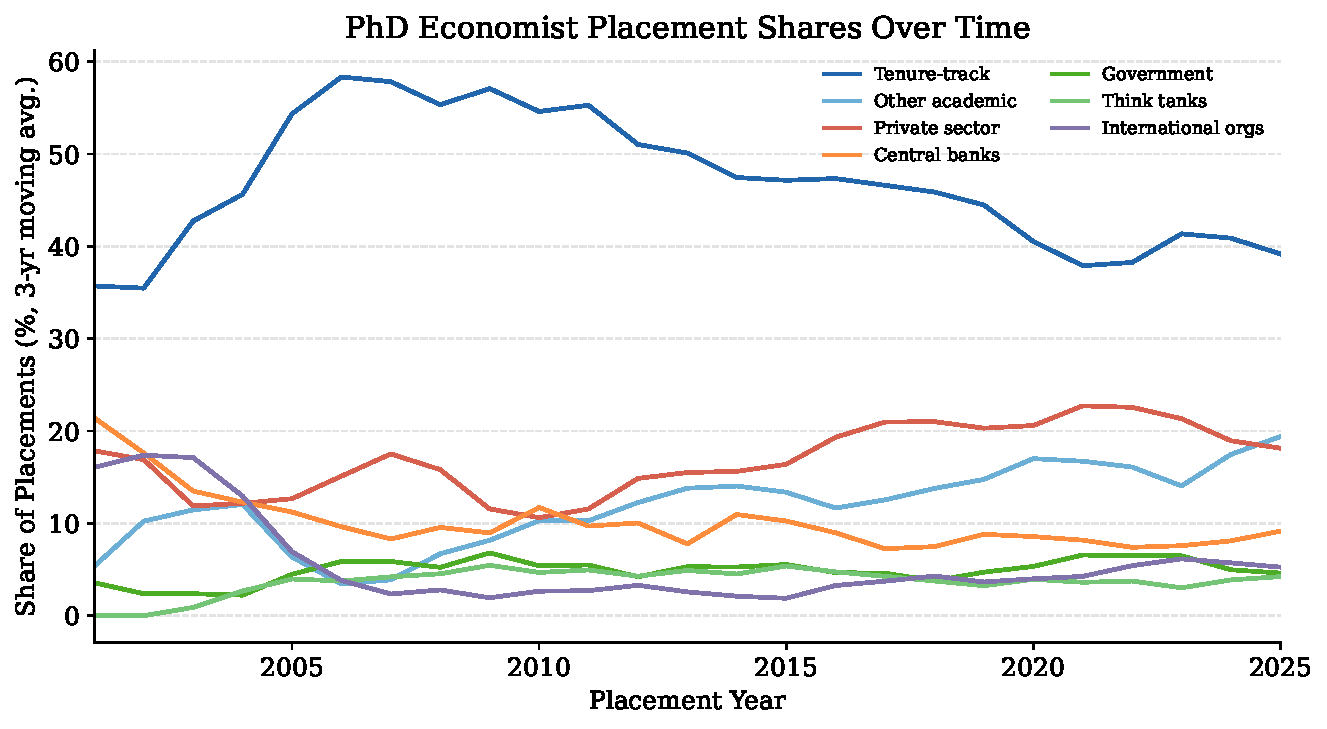
\includegraphics[width=0.90\textwidth]{placement_trends}
  \end{center}
  \begin{itemize}
    \item Tenure-track share declining since $\approx$2010; other academic rising
    \item Private sector growing steadily; central bank placements relatively stable
  \end{itemize}
\end{frame}

\begin{frame}{Placement Shares: EconPhDPlacements vs.\ Foster et al.\ (2023, JEP)}
  \begin{center}
    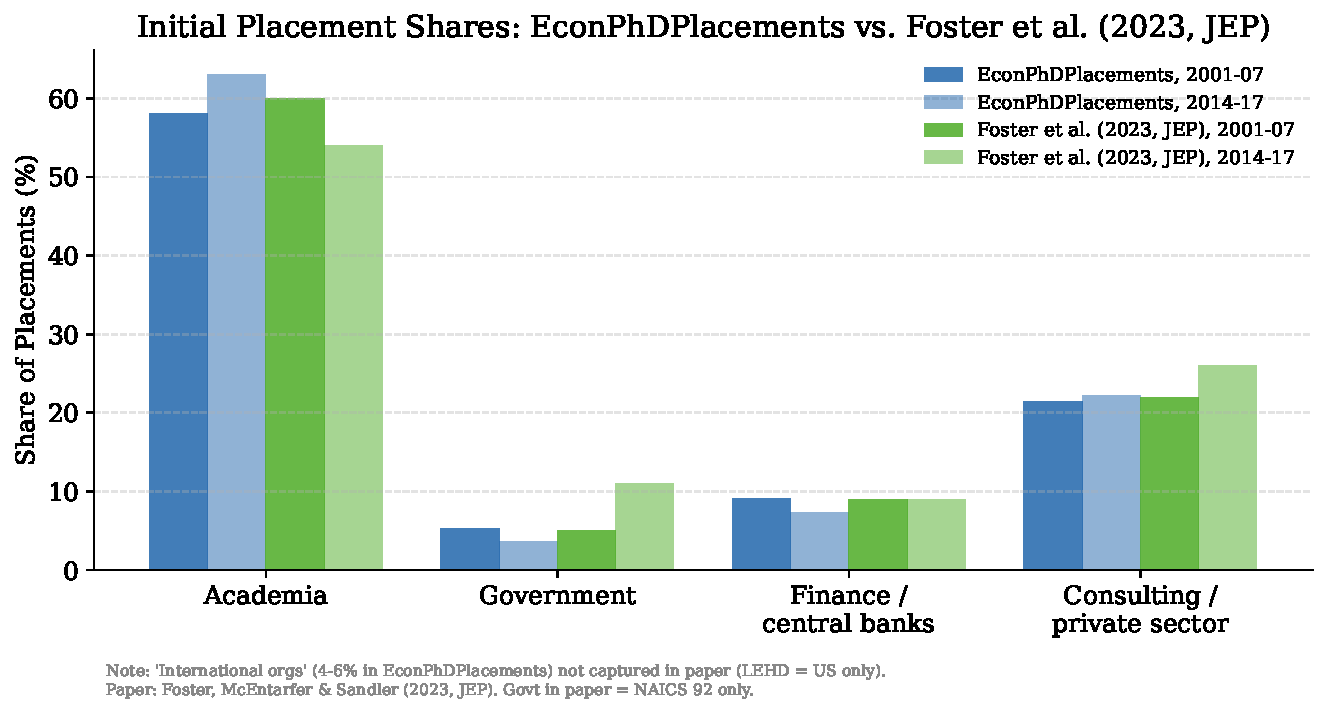
\includegraphics[width=0.88\textwidth]{placement_comparison}
  \end{center}
\end{frame}

\begin{frame}{Reconciling the Differences}
  \textbf{Our academia share (63\%, 2014--17) is higher than paper's (54\%, all programs):}
  \vspace{0.3em}
  \begin{itemize}
    \item Our 44 programs skew toward \textbf{top research universities} ---
          even for top-5 programs, paper shows 58.6\%
    \item Placement website data = \textbf{announced} initial placements;
          LEHD = actual employment (captures people who planned academia but moved)
    \item International programs in our sample (Stockholm, UBC, \ldots) may have
          higher academic placement rates
  \end{itemize}
  \vspace{0.5em}
  \textbf{Our government share (3.6\%, 2014--17) is lower than paper's (11\%):}
  \vspace{0.3em}
  \begin{itemize}
    \item Top programs go to government less (paper's top-5: 8.6\%; others: 11.4\%)
    \item Government placements may be under-reported on department websites
    \item Paper's government includes all levels (federal + state/local, NAICS 92)
  \end{itemize}
\end{frame}

\begin{frame}{Female Share by Sector: EconPhDPlacements vs.\ Foster et al.}
  \begin{center}
    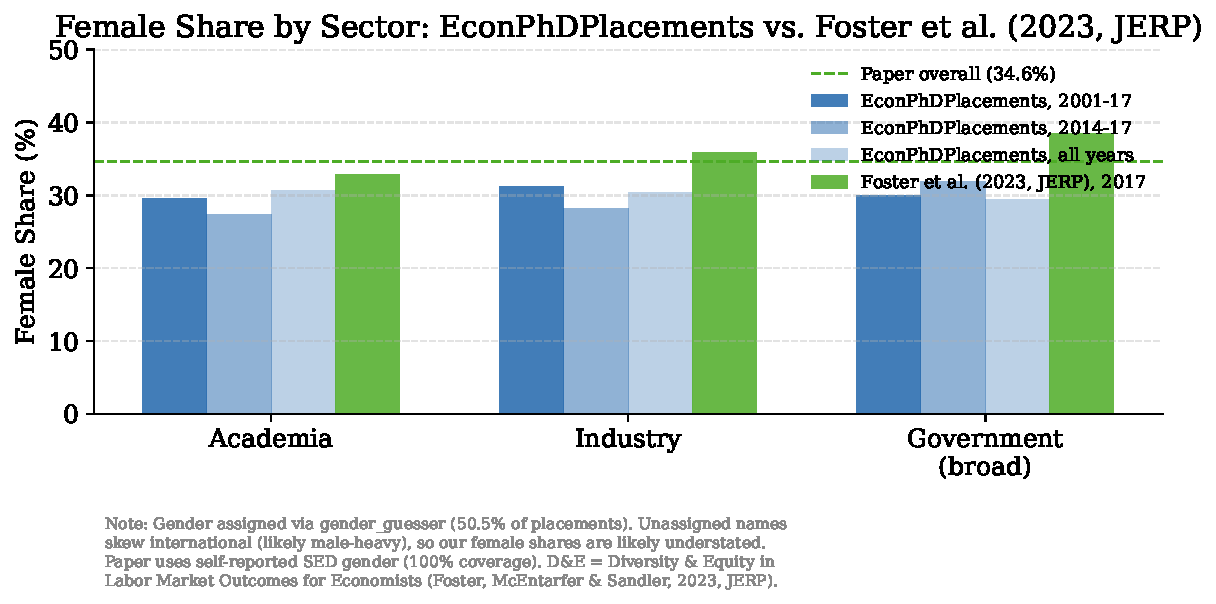
\includegraphics[width=0.88\textwidth]{female_sector_comparison}
  \end{center}
\end{frame}

\begin{frame}{Female Share in Placements: Caveats and Takeaways}
  \textbf{Our estimates (29--32\%) are below the paper's (33--38\%):}
  \vspace{0.3em}
  \begin{itemize}
    \item \textbf{Gender assignment gap:} only 51\% assigned; unassigned names
          are disproportionately international and likely male-heavy
          $\Rightarrow$ our female shares are understated by an unknown amount
    \item \textbf{Initial placements vs.\ cross-section:} paper shows the 2017
          stock of employed PhD economists (includes earlier cohorts with higher female
          retention); ours shows the flow of new placements
    \item \textbf{Ranking within sectors is preserved:}
          government $>$ industry $>$ academia in both datasets
  \end{itemize}
  \vspace{0.3em}
  \textbf{Next step:} use gender-specific name databases (e.g., Social Security
  Administration data, genderize.io) to improve coverage for international names
\end{frame}

% =============================================================================
\section{Summary}
% =============================================================================

\begin{frame}{Summary}
  \textbf{Federal salary (FedsDataCenter, FY2015--2024):}
  \begin{itemize}
    \item Raw median gender gap: 0--3.4\%, broadly consistent with Foster et al.\ (2020)
    \item Gap is entirely between-grade, not within-grade; BEA, Census, BLS show
          female salary \textit{advantage} at median
    \item Female share rising: 32\% $\to$ 34\%; gap re-widened post-2021
  \end{itemize}
  \vspace{0.4em}
  \textbf{PhD placements (econphdplacements.com, 1991--2025):}
  \begin{itemize}
    \item Sample skews toward top programs; academia share higher than national average
    \item Government placements under-represented vs.\ LEHD-based paper
    \item International orgs (4--6\%) visible here but absent from LEHD data
    \item Female share understated due to gender assignment coverage;
          ordering across sectors preserved
  \end{itemize}
  \vspace{0.4em}
  \textbf{Next steps:}
  \begin{itemize}
    \item Improve gender assignment for international names
    \item Link placement and salary data on individual economists
    \item Extend to regression-based gap estimates controlling for grade/agency
  \end{itemize}
\end{frame}

\begin{frame}[allowframebreaks]{References}
  \small
  \begin{itemize}
    \item Foster, L., Manzella, J., McEntarfer, E., \& Sandler, D.H.\ (2020).
          ``Employment and Earnings for Federal Government Economists: Empirical
          Evidence by Gender and Race.''
          \textit{AEA Papers and Proceedings}, 110, 210--214.
    \item Foster, L., McEntarfer, E., \& Sandler, D.H.\ (2023).
          ``Diversity and Equity in Labor Market Outcomes for Economists.''
          \textit{Journal of Economics, Race, and Policy}.
    \item Foster, L., McEntarfer, E., \& Sandler, D.H.\ (2023).
          ``Early Career Paths of Economists Inside and Outside of Academia.''
          \textit{Journal of Economic Perspectives}, 37(4), 231--250.
    \item Data: FedsDataCenter.com (OPM federal salary data, FY2015--2024)
    \item Data: econphdplacements.com (PhD economist placement data, 1991--2025)
  \end{itemize}
\end{frame}

\end{document}
